\documentclass[12pt, onside]{article}

\usepackage{fontspec,unicode-math} % Required for using utf8 characters in math mode
\usepackage{parskip}% Extra interlining
\usepackage[margin=0.8in]{geometry}    % Margins
\usepackage[spanish]{babel}
\usepackage{hyperref}
\usepackage{xcolor}
\usepackage{graphicx}
\usepackage[binary-units=true]{siunitx}
\usepackage{multirow}
\usepackage{mathtools}
\usepackage{array}
\usepackage{physics}
\usepackage{cleveref}
\usepackage{float}
\usepackage[toc,page]{appendix}


% Header and Footer
\usepackage{fancyhdr}
\setlength\headheight{30pt}
\pagestyle{fancy}
\renewcommand{\headrulewidth}{0.4pt}
\fancyhead{}
\fancyhead[L]{
    \textbf{Numerical implementation of the two-body problem}
}
\fancyhead[R]{
    Emilio Domínguez Sánchez
}
\fancyfoot{}
\fancyfoot[C]{\thepage}

% Code Listings Configuration File

\usepackage{listings}
% \renewcommand{\lstlistingname}{Código}
\crefname{lstlisting}{listing}{listings}
\Crefname{lstlisting}{Listing}{Listings}
% \renewcommand{\lstlistlistingname}{Índice de códigos}


\definecolor{background}{rgb}{0.99,0.99,0.99}
\definecolor{mygreen}{rgb}{0.1,0.6,0.1}
\definecolor{mygray}{rgb}{0.5,0.5,0.5}
\definecolor{mymauve}{rgb}{0.58,0,0.82}

\definecolor{codeback}{rgb}{0.85,0,0.85}

\lstset{ 
  title=File \lstname,          % show the filename of files included with \lstinputlisting; also try caption instead of title
  caption=File \texttt{\lstname},
  captionpos=t,                    % sets the caption-position (b/t)
  frame=TBLR,      	               % adds a frame around the code
  rulecolor=\color{black},         % if not set, the frame-color may be changed on line-breaks within not-black text (e.g. comments (green here))
  numbers=left,                    % where to put the line-numbers; possible values are (none, left, right)
  numbersep=10pt,                  % how far the line-numbers are from the code
  stepnumber=0,                    % the step between two line-numbers. If it's 1, each line will be numbered
  backgroundcolor=\color{background},
  numberstyle=\small\color{mygray},% the style that is used for the line-numbers
  basicstyle=\footnotesize\selectfont, % the size/type of the fonts that are used for the code
  keywordstyle=\color{mygreen},       % keyword style
  commentstyle=\color{blue},    % comment style
  stringstyle=\color{mymauve},     % string literal style
  breakatwhitespace=false,         % sets if automatic breaks should only happen at whitespace
  breaklines=true,                 % sets automatic line breaking
  keepspaces=true,                 % keeps spaces in text, useful for keeping indentation of code (possibly needs columns=flexible)
  showstringspaces=false,          % underline spaces within strings only
  showspaces=false,                % show spaces everywhere adding particular underscores; it overrides 'showstringspaces'
  showtabs=false,                  % show tabs within strings adding particular underscores
  tabsize=2,	                   % sets default tabsize to 2 spaces
  language=Matlab,                    % the language of the code
  morekeywords={arenstorf},            % if you want to add more keywords to the set
  deletekeywords={},            % if you want to delete keywords from the given language
  % escapeinside={----}{----},          % if you want to add LaTeX within your code
  extendedchars=true,              % lets you use non-ASCII characters; for 8-bits encodings only, does not work with UTF-8
  literate=
  {á}{{\'a}}1 {é}{{\'e}}1 {í}{{\'i}}1 {ó}{{\'o}}1 {ú}{{\'u}}1
  {Á}{{\'A}}1 {É}{{\'E}}1 {Í}{{\'I}}1 {Ó}{{\'O}}1 {Ú}{{\'U}}1
  {à}{{\`a}}1 {è}{{\`e}}1 {ì}{{\`i}}1 {ò}{{\`o}}1 {ù}{{\`u}}1
  {À}{{\`A}}1 {È}{{\'E}}1 {Ì}{{\`I}}1 {Ò}{{\`O}}1 {Ù}{{\`U}}1
  {ä}{{\"a}}1 {ë}{{\"e}}1 {ï}{{\"i}}1 {ö}{{\"o}}1 {ü}{{\"u}}1
  {Ä}{{\"A}}1 {Ë}{{\"E}}1 {Ï}{{\"I}}1 {Ö}{{\"O}}1 {Ü}{{\"U}}1
  {â}{{\^a}}1 {ê}{{\^e}}1 {î}{{\^i}}1 {ô}{{\^o}}1 {û}{{\^u}}1
  {Â}{{\^A}}1 {Ê}{{\^E}}1 {Î}{{\^I}}1 {Ô}{{\^O}}1 {Û}{{\^U}}1
  {œ}{{\oe}}1 {Œ}{{\OE}}1 {æ}{{\ae}}1 {Æ}{{\AE}}1 {ß}{{\ss}}1
  {ű}{{\H{u}}}1 {Ű}{{\H{U}}}1 {ő}{{\H{o}}}1 {Ő}{{\H{O}}}1
  {ç}{{\c c}}1 {Ç}{{\c C}}1 {ø}{{\o}}1 {å}{{\r a}}1 {Å}{{\r A}}1
  {€}{{\euro}}1 {£}{{\pounds}}1 {«}{{\guillemotleft}}1
  {»}{{\guillemotright}}1 {ñ}{{\~n}}1 {Ñ}{{\~N}}1 {¿}{{?`}}1
}



\newcommand{\R}{{\mathbb{R}}}
% \renewcommand{\dv}{\prime}
\newcommand{\ddv}{\dprime}
\renewcommand{\dv}{\prime}
\newcommand{\inner}[2]{\left\langle #1, \; #2 \right\rangle}
\newcommand{\vr}{{\vb{r}}}
\newcommand{\vx}{{\vb{x}}}
\newcommand{\CM}{{\operatorname{CM}}}

\begin{document}
\begin{titlepage}
    \begin{center}
        \vspace*{1cm}
        
        \Huge \textbf{Arenstorf Orbit}
        
        \vspace{0.5cm}
        \LARGE Implementation of iterative methods
        
        \vspace{0.5cm}
        
        \Large Assignment for \\ Métodos Numéricos de las Ecuaciones Diferenciales
        
        \vspace{0.5cm}
   		
        \vfill
        
        %Obor XY
        \vspace{0.8cm}
        \Large
            \begin{flushright}
              	\begin{tabular}{lr}
                  Author: & Emilio Domínguez Sánchez\\
                  Due Date: & 12th of November of 2020\\
                \end{tabular}
            \end{flushright}
        \vspace{0.5cm}
        
    \end{center}
\end{titlepage}

\newpage
\tableofcontents
\newpage

\section{Introduction}

    Richard Arenstorf discovered a stable periodic orbit between the Earth and the Moon
which was later used as the basis for Apollo missions.

    In this paper, we work with the initial value problem corresponding to Arenstorf's orbit
and compute the solution with different iterative methods.

\section{Problem description}

    This an instace of the three body problem.
Two of the objects, the Earth and the Moon, are orbiting in a plane.
The third one, our satellite, of negligible mass,
is only affected by the attraction of this two large bodies.

\subsection{Initial Value Problem}

    The system of equations that govern the system are given by
%
\begin{gather*}
    \begin{alignedat}{2}
        x\ddv &= x + 2y\dv - M\frac{x+m}{D_1}& - m&\frac{x-M}{D_2} \\
        y\ddv &= y + 2x\dv - M\frac{y}{D_1}& - m&\frac{y}{D_2} \\
    \end{alignedat} \\
    \begin{alignedat}{1}
        D_1 = &((x+m)^2 + y^2)^{\frac{3}{2}} \\
        D_2 = &((x-m)^2 + y^2)^{\frac{3}{2}} \\
    \end{alignedat} \\
    \begin{alignedat}{1}
        m &= \num{0.012277471} \\
        M &= 1-m \\
    \end{alignedat}
\end{gather*}
%
where $M$ and $m$ are the mass of the Earth and the Moon respectively.

    The initial conditions are taken normalized to the problem
to increase the numerical accuracy.
For example, the distance between the Earth and the Moon is $1$ and
the sum of masses of the Earth and the Moon is also $1$.
%
\begin{alignat*}{2}
    x(0) &= (\num{0.994} & 0) \\
    y(0) &= (0 & \num{-2.001585106}) \\
\end{alignat*}

\section{Objective}

    The objective is tracing the orbit for two cycles
using three fixed step methods:
Euler's method, the modified version of Euler's method and the Runge-Kutta $4$ Method;
as well as two adaptative steps methods: Felhberg's method and
Richardson's extrapolation with variation of the step of the Runge-Kutta $4$ method.
We are interested in obtaining the best possible approximation with each method
and the number of evaluations and the running time of each method.

\section{Implementation}

\subsection{General considerations}

    To determine when the methods should stop
I decided to compare the points with the starting point.
However, we need to stop at the second turn.
Some initial tries with a good method (like RK4) show that
the time taken in a complete turn is approximately $17$ time units.
Hence, the implementations use a lambda function (usually inlined in Julia) that checks
this giving a tolerance called \lstinline!closing_err!.
This value is different depending on the methods,
because some where able to obtain better results than the rest.

\begin{lstlisting}[
    gobble=4,
    caption=Stop condition for the methods,
        basicstyle=\scriptsize
]
    (t, x) ->
        t > 20 && norm(Arenstorf.p0 .- last(x)[1:2]) < closing_err || t > stop_time,
\end{lstlisting}

    It was also necessary to have a means of measuring the error of each solution.
I measured the distance from the method's to the initial points after two iterations
and that same distance when we interpolate the solution based on the last $5$ points
to obtain what would be the exact $x$-coordinate when the $y$-coordinate is $0$,
as in the beginning.
I reused the code for Hermite's interpolation from previous assignments.

\begin{lstlisting}[
    gobble=4,
    caption=Code corresponding to Hermite's interpolation in the tests,
    basicstyle=\scriptsize
]
    n = length(x)
    last5x = [p[1] for p in x[n-4:n]]
    last5y = [p[2] for p in x[n-4:n]]
    closingx = Interpolation.hermite(last5y, last5x, 0)
    print("\tDistance from interpolated closing point to start point: ",
          "$(abs(closingx - Arenstorf.p0[1]))\n")
\end{lstlisting}

\subsection{Plotting and building gifs from the solutions}

    In order to build gifs (or plots) for the solutions, we must use the solutions computed.
However, we have usually computed a lot of points.
This number of points makes it possible to use the solution in other contexts
or draw it smoothly,
but processing a frame for each point would require a lot of computation time.
Furthermore, it would be wrong for mixed step methods,
because each frame would not correspond to the same fraction of time.
Hence, plotting or drawing a frame every $k$ points is also wrong,
and if we do so,
we may be able to see some inconsistencies even in our plots.
Specifically, we could see some polygonals in the more complex parts of our drawing.
Instead, we must iterate over the time (with a fixed step) and plot/frame
all the points seen until that moment.

\begin{lstlisting}[
    gobble=4,
    caption=Creation of gifs in Julia,
    basicstyle=\scriptsize
]
    len = length(t)
    anim = Animation()
    i = 2
    for j = 0:0.05:t[len]
        while i < len && t[i] < j
            i += 1
        end
        # NaNs are used to avoid plotting more points for the Earth
        push!(p1, [(x[i][1], x[i][2]), (cos(2*π*t[i]/t[len]), sin(2*π*t[i]/t[len])), (NaN, NaN)])
        push!(p2, t[i], steps[i-1])
        plot(p1, p2)
        frame(anim)
    end
    gif(anim, "media/arenstorf/richardson.gif", fps = 15)
\end{lstlisting}

\subsection{Euler's Method}

\begin{figure}[H]
    \centering
    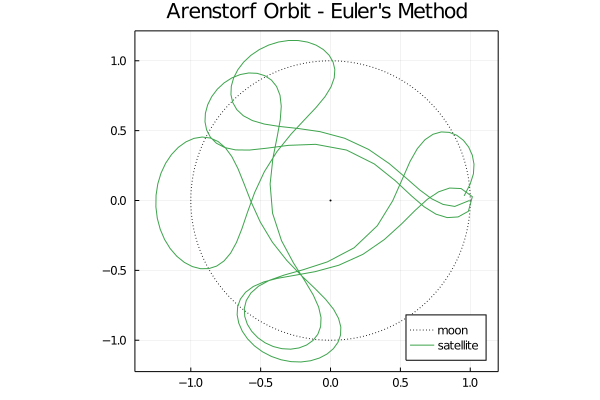
\includegraphics[width=0.8\textwidth]{media/arenstorf/euler.png}
    \caption{Graphical results for Euler's method.}
\end{figure}

    Euler's method is the worst of the tested.
We could say it behaved properly for one turn,
but the accumulated error was too big for the second turn in this problem.
I tried reducing the step to $\num{1e-6}$ with just one turn,
but the results were not favorable either.
In this case, there is no point in checking the distance given by interpolation,
because it is very clear that the orbit is deformed with respect to the original one.

\lstinputlisting{outputs/arenstorf/euler.txt}

\subsection{Modified Euler's Method}

\begin{figure}[H]
    \centering
    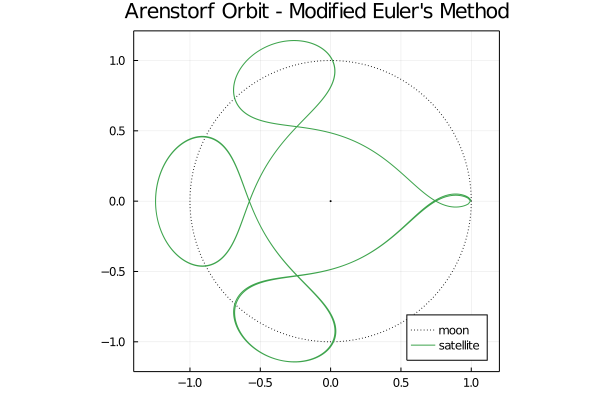
\includegraphics[width=0.7\textwidth]{media/arenstorf/mod_euler.png}
    \caption{Graphical results for the modified version of Euler's method.}
    \label{fig:mod_euler}
\end{figure}

    The modified version of Euler's method improved significantly with respect
to the original one.
In this case, I also needed to reduce significantly the step size to obtain better results.
I used the least step among all methods because I could obtain
a better solution with that step size,
which I was not able with Euler's method.
I did not reduce it more because the running time was already over $\SI{30}{\s}$.
This made me think that I needed to consider the performance of the iterative methods.
The conclusions will be presented later (\cref{sec:performance}).

    In this case, we can see in the plot (\cref{fig:mod_euler}) that the second cycle
is slightly different than the first one towards the end.
In the following methods, the differences will not be visible.
The method gave an error when closing the orbit of $\num{4e-3}$.
Because the initial point was almost at distance $1$, this error is also the relative error.
This means that even for an unstable problem like this one,
reducing the step size enough can provide reasonable results.
But then again,
the next methods achieve more in less time.

\lstinputlisting{outputs/arenstorf/mod_euler.txt}

\subsection{Runge Kutta $4$ Method}

\begin{figure}[H]
    \centering
    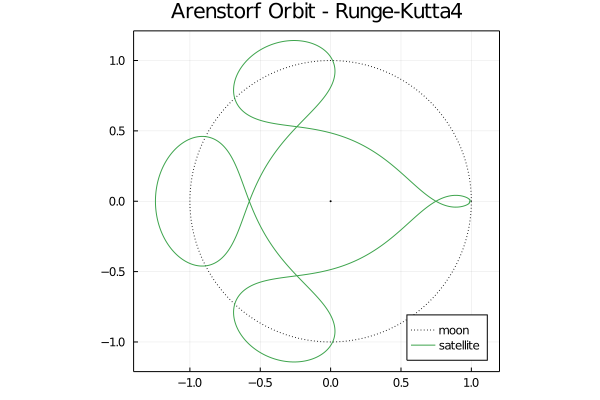
\includegraphics[width=0.8\textwidth]{media/arenstorf/rk4.png}
    \caption{Graphical results for the RK4 method.}
\end{figure}

    The RK4 is the first method for which we obtain a plot that
visually seems like a single cycle,
meaning that it approximates very well,
and a closing error of $\num{2.8e-8}$ (after interpolation).
However, we still need to use a very small step ($\num{1e-5}$) to obtain good results,
while with the adaptative methods,
the number of iterations, and therefore the running time,
decrease significantly.
The conclusion is that an approximation of order $4$ with steps of $\num{1e-5}$
gives good results for this problem,
but there are parts of the orbit where the system is more stable and we can use bigger steps.

\lstinputlisting{outputs/arenstorf/rk4.txt}

\subsection{Felhberg's method}

\begin{figure}[H]
    \centering
    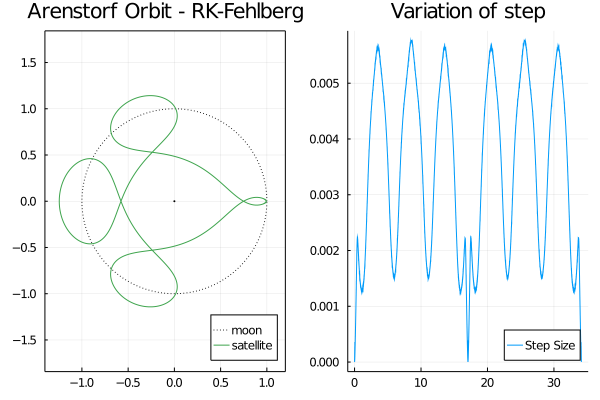
\includegraphics[width=0.95\textwidth]{media/arenstorf/fehlberg.png}
    \caption{Graphical results for Felhberg's method.}
\end{figure}

    I tweaked the values for Felhberg's method until I saw I could no longer decrease the
approximation error.
I was not able to reduce the closing error below $\num{1e-5}$,
even when I set the tolerance to $\num{1e-16}$,
something that also happened with Richardson's extrapolation.
Felhberg's was the best method for this problem,
the fastest (a little bit above one second in my hardware)
and the one that performed the least number of evaluations of the derivative function.

\lstinputlisting{outputs/arenstorf/fehlberg.txt}

\subsection{Richardson's extrapolation of the RK4 method}

\begin{figure}[H]
    \centering
    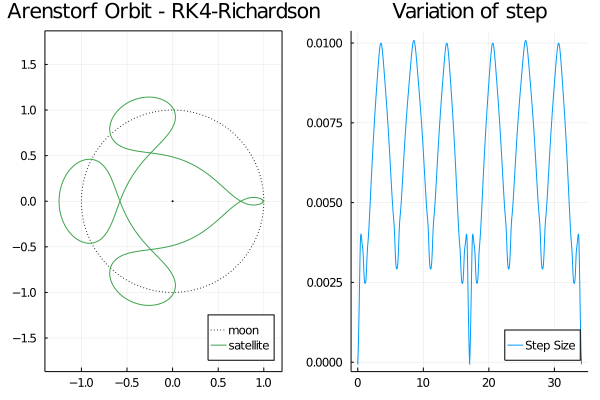
\includegraphics[width=0.95\textwidth]{media/arenstorf/richardson.png}
    \caption{Graphical results for Richardson's extrapolation of the RK4 method.}
\end{figure}

    The last method performed similarly to the previous one.
It also falls in the category of mixed step methods,
and as such it was much faster than the fixed step methods,
but it was slower and required more evaluations that Felhberg's method.
A slight improvement with respect to Fehlberg's method
is that the maximum step was slightly bigger, but so was the tolerance of the method.

\lstinputlisting{outputs/arenstorf/richardson.txt}

\section{Access to the code}

    The code at the moment of writting can be checked in my Git repository.
{\small
\url{https://github.com/useredsa/numeric-differential-equations/commit/c0c34ee66c30e19cf622e8280653d83207a0ce89}
}

    I recommend looking at the files
\href{https://github.com/useredsa/numeric-differential-equations/blob/c0c34ee66c30e19cf622e8280653d83207a0ce89/media/arenstorf/fehlberg.gif}{\lstinline{fehlberg.gif}}
and
\href{https://github.com/useredsa/numeric-differential-equations/blob/c0c34ee66c30e19cf622e8280653d83207a0ce89/media/arenstorf/richardson.gif}{\lstinline!richardson.gif!}
which show animations of the satellite, the moon and the step size
for both adaptative methods.

\end{document}
